\documentclass{standalone}
\usepackage{tikz}
\usetikzlibrary{patterns}
\usetikzlibrary{positioning}
\usetikzlibrary{patterns, positioning}
\usetikzlibrary{shapes.misc}
\usepackage[outline]{contour}
\contourlength{1.5pt} 
\usepackage[sfdefault]{ClearSans}

\begin{document}
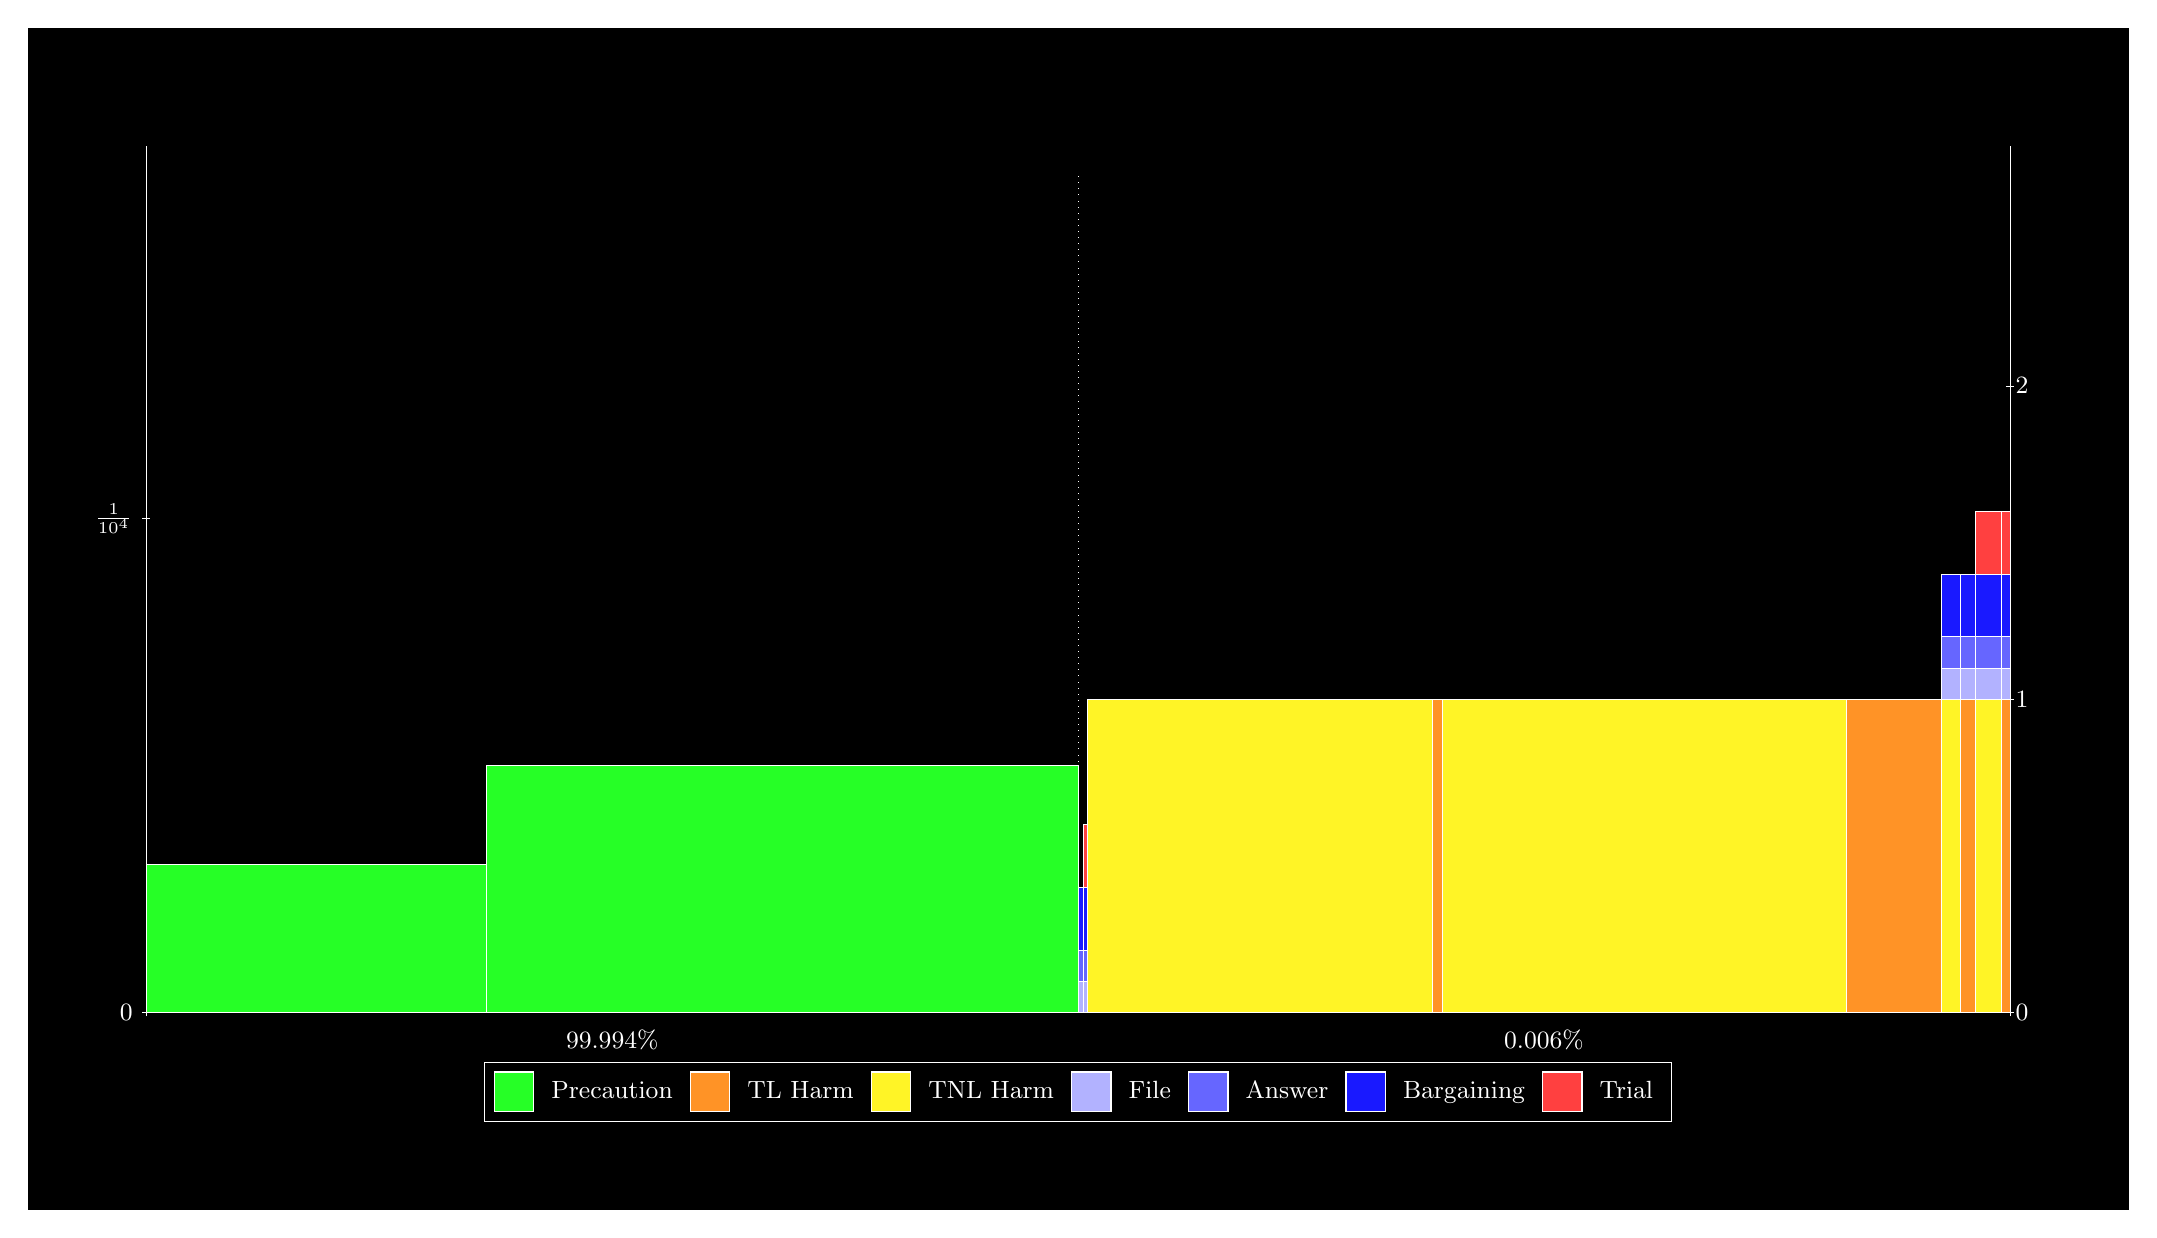
\begin{tikzpicture}
\draw[fill=black] (0,0) rectangle (26.667,15);
\draw[fill=green!85,draw=white,very thin] (1.5,2.5) rectangle (5.8205,4.3815);
\draw[fill=green!85,draw=white,very thin] (5.8205,2.5) rectangle (13.333,5.6359);
\draw[fill=green!85,draw=white,very thin] (13.333,2.5) rectangle (13.393,2.5001);
\draw[fill=blue!30,draw=white,very thin] (13.333,2.5001) rectangle (13.393,2.898);
\draw[fill=blue!60,draw=white,very thin] (13.333,2.898) rectangle (13.393,3.2958);
\draw[fill=blue!90,draw=white,very thin] (13.333,3.2958) rectangle (13.393,4.0916);
\draw[fill=green!85,draw=white,very thin] (13.393,2.5) rectangle (13.452,2.5001);
\draw[fill=blue!30,draw=white,very thin] (13.393,2.5001) rectangle (13.452,2.898);
\draw[fill=blue!60,draw=white,very thin] (13.393,2.898) rectangle (13.452,3.2958);
\draw[fill=blue!90,draw=white,very thin] (13.393,3.2958) rectangle (13.452,4.0916);
\draw[fill=red!75,draw=white,very thin] (13.393,4.0916) rectangle (13.452,4.8873);
\draw[fill=green!85,draw=white,very thin] (13.452,2.5) rectangle (17.834,2.5001);
\draw[fill=yellow!85,draw=white,very thin] (13.452,2.5001) rectangle (17.834,6.4788);
\draw[fill=green!85,draw=white,very thin] (17.834,2.5) rectangle (17.954,2.5001);
\draw[fill=orange!85,draw=white,very thin] (17.834,2.5001) rectangle (17.954,6.4788);
\draw[fill=green!85,draw=white,very thin] (17.954,2.5) rectangle (23.094,2.5002);
\draw[fill=yellow!85,draw=white,very thin] (17.954,2.5002) rectangle (23.094,6.4788);
\draw[fill=green!85,draw=white,very thin] (23.094,2.5) rectangle (24.292,2.5002);
\draw[fill=orange!85,draw=white,very thin] (23.094,2.5002) rectangle (24.292,6.4788);
\draw[fill=green!85,draw=white,very thin] (24.292,2.5) rectangle (24.541,2.5001);
\draw[fill=yellow!85,draw=white,very thin] (24.292,2.5001) rectangle (24.541,6.4788);
\draw[fill=blue!30,draw=white,very thin] (24.292,6.4788) rectangle (24.541,6.8766);
\draw[fill=blue!60,draw=white,very thin] (24.292,6.8766) rectangle (24.541,7.2745);
\draw[fill=blue!90,draw=white,very thin] (24.292,7.2745) rectangle (24.541,8.0702);
\draw[fill=green!85,draw=white,very thin] (24.541,2.5) rectangle (24.73,2.5001);
\draw[fill=orange!85,draw=white,very thin] (24.541,2.5001) rectangle (24.73,6.4788);
\draw[fill=blue!30,draw=white,very thin] (24.541,6.4788) rectangle (24.73,6.8766);
\draw[fill=blue!60,draw=white,very thin] (24.541,6.8766) rectangle (24.73,7.2745);
\draw[fill=blue!90,draw=white,very thin] (24.541,7.2745) rectangle (24.73,8.0702);
\draw[fill=green!85,draw=white,very thin] (24.73,2.5) rectangle (25.056,2.5001);
\draw[fill=yellow!85,draw=white,very thin] (24.73,2.5001) rectangle (25.056,6.4788);
\draw[fill=blue!30,draw=white,very thin] (24.73,6.4788) rectangle (25.056,6.8766);
\draw[fill=blue!60,draw=white,very thin] (24.73,6.8766) rectangle (25.056,7.2745);
\draw[fill=blue!90,draw=white,very thin] (24.73,7.2745) rectangle (25.056,8.0702);
\draw[fill=red!75,draw=white,very thin] (24.73,8.0702) rectangle (25.056,8.8659);
\draw[fill=green!85,draw=white,very thin] (25.056,2.5) rectangle (25.167,2.5001);
\draw[fill=orange!85,draw=white,very thin] (25.056,2.5001) rectangle (25.167,6.4788);
\draw[fill=blue!30,draw=white,very thin] (25.056,6.4788) rectangle (25.167,6.8766);
\draw[fill=blue!60,draw=white,very thin] (25.056,6.8766) rectangle (25.167,7.2745);
\draw[fill=blue!90,draw=white,very thin] (25.056,7.2745) rectangle (25.167,8.0702);
\draw[fill=red!75,draw=white,very thin] (25.056,8.0702) rectangle (25.167,8.8659);
\draw[white,very thin] (1.5,2.5) -- (1.5,13.5);
\draw[white,very thin] (1.45,2.5) -- (1.55,2.5);
\node[font=\small,text=white, anchor=east] at (1.45, 2.5) {0};
\draw[white,very thin] (1.45,8.7718) -- (1.55,8.7718);
\node[font=\small,text=white, anchor=east] at (1.45, 8.7718) {$\frac{1}{10^{4}}$};

\draw[white,dotted,very thin] (13.333,2.83) -- (13.333,13.17);
\draw[white,very thin] (25.167,2.5) -- (25.167,13.5);
\draw[white,very thin] (25.117,2.5) -- (25.217,2.5);
\node[font=\small,text=white, anchor=west] at (25.117, 2.5) {0};
\draw[white,very thin] (25.117,6.4786) -- (25.217,6.4786);
\node[font=\small,text=white, anchor=west] at (25.117, 6.4786) {1};
\draw[white,very thin] (25.117,10.457) -- (25.217,10.457);
\node[font=\small,text=white, anchor=west] at (25.117, 10.457) {2};

\draw[white,very thin] (1.5,2.5) -- (25.167,2.5);
\draw[white,very thin] (1.5,2.45) -- (1.5,2.55);
\node[font=\small,text=white, anchor=north] at (1.5, 2.45) {};
\draw[white,very thin] (25.167,2.45) -- (25.167,2.55);
\node[font=\small,text=white, anchor=north] at (25.167, 2.45) {};

\node[font=\small,text=white,anchor=south] at (7.4167, 1.9) {99.994\%};
\node[font=\small,text=white,anchor=south] at (19.25, 1.9) {0.006\%};
\draw (13.3333,2.5) node (B) {};
\begin{scope}[align=center]
\matrix[scale=0.5,draw=white,below=0.5cm of B,nodes={draw},column sep=0.1cm]{
\node[rectangle,draw,minimum width=0.5cm,minimum height=0.5cm,fill=green!85]{}; & \node[draw=none,font=\small,text=white]{Precaution}; &
\node[rectangle,draw,minimum width=0.5cm,minimum height=0.5cm,fill=orange!85]{}; & \node[draw=none,font=\small,text=white]{TL Harm}; &
\node[rectangle,draw,minimum width=0.5cm,minimum height=0.5cm,fill=yellow!85]{}; & \node[draw=none,font=\small,text=white]{TNL Harm}; &
\node[rectangle,draw,minimum width=0.5cm,minimum height=0.5cm,fill=blue!30]{}; & \node[draw=none,font=\small,text=white]{File}; &
\node[rectangle,draw,minimum width=0.5cm,minimum height=0.5cm,fill=blue!60]{}; & \node[draw=none,font=\small,text=white]{Answer}; &
\node[rectangle,draw,minimum width=0.5cm,minimum height=0.5cm,fill=blue!90]{}; & \node[draw=none,font=\small,text=white]{Bargaining}; &
\node[rectangle,draw,minimum width=0.5cm,minimum height=0.5cm,fill=red!75]{}; & \node[draw=none,font=\small,text=white]{Trial}; \\\\
};\end{scope}

\end{tikzpicture}
\end{document}